\documentclass[10pt]{beamer}
\usetheme{Madrid}

\usepackage[utf8]{inputenc}
\usepackage[T1]{fontenc}
\usepackage[brazil]{babel}
\usepackage{booktabs}
\usepackage{multirow}
\usepackage{graphicx}
\usepackage{amsmath}
\usepackage{array}
\usepackage{colortbl}

\definecolor{cefetblue}{RGB}{0,68,124}
\setbeamercolor{structure}{fg=cefetblue}

\title[Predição de Diabetes Tipo 2]{Predição de Diabetes Mellitus Tipo 2 Utilizando Técnicas de Inteligência Computacional}
\subtitle{Uma Análise Comparativa}
\author[Rafael et al.]{Rafael A. S. Ferreira \and João M. G. Lisboa \and Gabriel V. Silva \\[0.3em] CEFET-MG --- Inteligência Computacional}
\institute[CEFET-MG]{Centro Federal de Educação Tecnológica de Minas Gerais \\ Campus V --- Divinópolis}
\date{Junho de 2026}

\begin{document}

% ================================================================
% SLIDE DE APRESENTAÇÃO
% ================================================================
\frame{\titlepage}

% ================================================================
% SUMÁRIO
% ================================================================
\begin{frame}{Sumário}
    \tableofcontents
\end{frame}

% ================================================================
\section{Introdução}
% ================================================================
\begin{frame}{Contexto e Motivação}
    \begin{itemize}
        \item O Diabetes Mellitus Tipo 2 (DMT2) é uma das principais epidemias de saúde do século XXI.
        \item Mais de \textbf{537 milhões} de adultos viviam com a doença em 2021 (IDF).
        \item No Brasil, cerca de \textbf{16,8 milhões} de pessoas são afetadas.
        \item Até 50\% dos casos permanecem não diagnosticados por anos.
        \item A predição precoce permite intervenções preventivas e redução de custos hospitalares.
    \end{itemize}
    \vspace{0.3cm}
    \begin{block}{Por que Inteligência Computacional?}
        A relação entre fatores de risco e diabetes é \textbf{não-linear e multivariada}, tornando-a adequada para técnicas de Aprendizado de Máquina.
    \end{block}
\end{frame}

\begin{frame}{Objetivo}
    Realizar uma análise comparativa sistemática de quatro algoritmos de Inteligência Computacional para predição de DMT2:
    \vspace{0.3cm}
    \begin{columns}
        \begin{column}{0.48\textwidth}
            \begin{itemize}
                \item \textbf{MLP} -- Multi-Layer Perceptron
                \item \textbf{SVM} -- Support Vector Machine
            \end{itemize}
        \end{column}
        \begin{column}{0.48\textwidth}
            \begin{itemize}
                \item \textbf{Random Forest}
                \item \textbf{Regressão Logística}
            \end{itemize}
        \end{column}
    \end{columns}
    \vspace{0.4cm}
    \begin{alertblock}{Foco}
        Avaliação rigorosa sob condições experimentais uniformes: mesma divisão dos dados, busca em grade de hiperparâmetros, balanceamento com SMOTE e métricas apropriadas para dados desbalanceados.
    \end{alertblock}
\end{frame}

% ================================================================
\section{Dataset e Pré-processamento}
% ================================================================
\begin{frame}{Dataset PIMA Indians Diabetes}
    \begin{itemize}
        \item \textbf{Fonte:} UCI Machine Learning Repository.
        \item \textbf{Amostras:} 768 mulheres da tribo Pima Indian (Arizona, EUA), idade $\geq$ 21 anos.
        \item \textbf{Atributos:} 8 variáveis numéricas preditivas.
        \item \textbf{Alvo:} presença (1) ou ausência (0) de DMT2.
        \item \textbf{Desbalanceamento:} 65,1\% negativos e 34,9\% positivos.
    \end{itemize}
    \vspace{0.2cm}
    \centering
    \footnotesize
    \begin{tabular}{@{}llc@{}}
        \toprule
        \textbf{Atributo} & \textbf{Descrição} & \textbf{Zeros impossíveis} \\
        \midrule
        NumGestacoes & Número de gestações & --- \\
        Glicose & Concentração plasmática de glicose & 5 \\
        Pressão Arterial & Pressão diastólica & 35 \\
        Espessura da Pele & Dobra cutânea do tríceps & 227 \\
        Insulina & Nível sérico de insulina & 374 \\
        IMC & Índice de Massa Corporal & 11 \\
        Pedigree & Histórico familiar & --- \\
        Idade & Idade em anos & --- \\
        \bottomrule
    \end{tabular}
\end{frame}

\begin{frame}{Pipeline de Pré-processamento}
    \begin{enumerate}
        \item \textbf{Tratamento de zeros impossíveis:} substituídos por NaN e imputados pela mediana do treino.
        \item \textbf{Divisão estratificada:} 60\% treino (460), 20\% validação (154), 20\% teste (154).
        \item \textbf{Padronização:} \texttt{StandardScaler} ajustado apenas no treino.
        \item \textbf{Balanceamento:} SMOTE apenas no treino (300/300 amostras).
    \end{enumerate}
    \vspace{0.3cm}
    \centering
    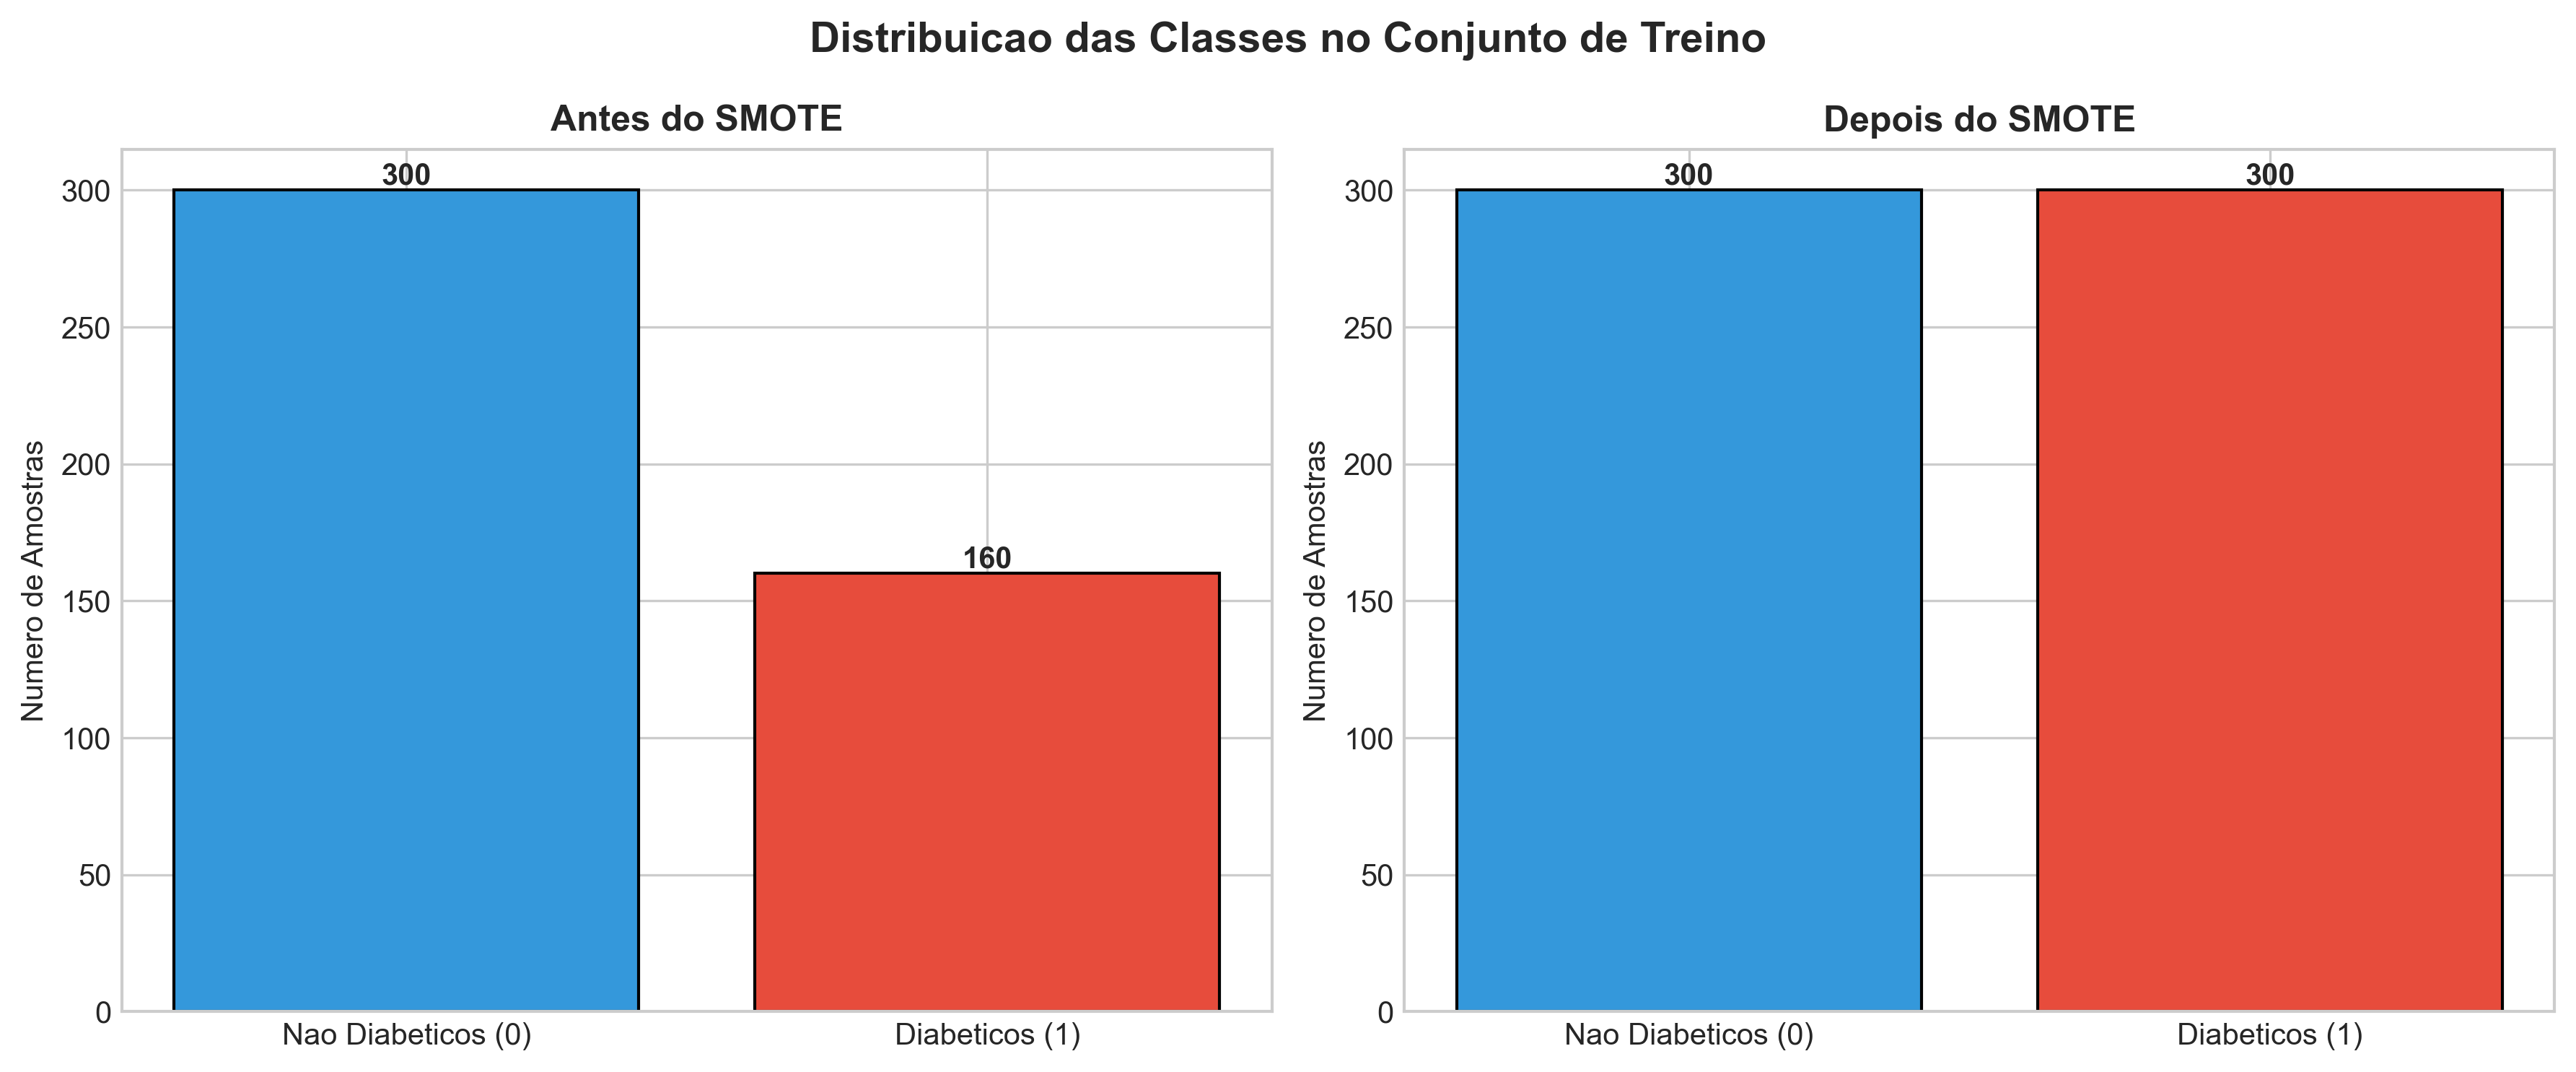
\includegraphics[width=0.85\textwidth,height=0.45\textheight,keepaspectratio]{../figuras_diabetes/02_distribuicao_classes.png}
\end{frame}

% ================================================================
\section{Algoritmos e Metodologia}
% ================================================================
\begin{frame}{Algoritmos Avaliados}
    \begin{columns}
        \begin{column}{0.48\textwidth}
            \textbf{MLP}\\
            \footnotesize Rede neural feedforward com backpropagation; capaz de capturar relações não-lineares complexas.
            \vspace{0.3cm}

            \textbf{SVM}\\
            \footnotesize Busca o hiperplano de separação ótimo; kernel RBF projeta dados para espaços de maior dimensionalidade.
        \end{column}
        \begin{column}{0.48\textwidth}
            \textbf{Random Forest}\\
            \footnotesize Ensemble de árvores de decisão via \textit{bagging}; robusto contra overfitting e fornece importância de variáveis.
            \vspace{0.3cm}

            \textbf{Regressão Logística}\\
            \footnotesize Modelo linear generalizado altamente interpretável, com regularização L1/L2 integrada.
        \end{column}
    \end{columns}
\end{frame}

\begin{frame}{Configuração dos Experimentos}
    \begin{itemize}
        \item \textbf{Seleção de hiperparâmetros:} GridSearchCV com validação cruzada de 5 folds.
        \item \textbf{Métrica de otimização:} F1-Score.
        \item \textbf{Repetições:} 10 execuções independentes para MLP e Random Forest.
        \item \textbf{Métricas de avaliação:} acurácia, precisão, revocação, F1-Score e AUC-ROC.
    \end{itemize}
    \vspace{0.3cm}
    \centering
    \footnotesize
    \begin{tabular}{@{}lll@{}}
        \toprule
        \textbf{Modelo} & \textbf{Principais parâmetros testados} & \textbf{Melhor F1 (CV)} \\
        \midrule
        MLP & camadas, ativação, learning rate & 0,778 \\
        SVM & C, kernel, gamma & 0,793 \\
        RF & n\_estimators, max\_depth, min\_samples\_split & 0,822 \\
        LogReg & C, solver & 0,757 \\
        \bottomrule
    \end{tabular}
\end{frame}

% ================================================================
\section{Resultados}
% ================================================================
\begin{frame}{Resultados de Desempenho}
    \centering
    \footnotesize
    \begin{tabular}{@{}lccccc@{}}
        \toprule
        \textbf{Modelo} & \textbf{Acurácia} & \textbf{Precisão} & \textbf{Revocação} & \textbf{F1} & \textbf{AUC-ROC} \\
        \midrule
        MLP & 0,718 $\pm$ 0,012 & 0,587 $\pm$ 0,017 & 0,667 $\pm$ 0,050 & 0,623 $\pm$ 0,023 & 0,812 $\pm$ 0,007 \\
        SVM & 0,721 & 0,604 & 0,593 & 0,598 & 0,792 \\
        RF & 0,733 $\pm$ 0,012 & 0,619 $\pm$ 0,016 & 0,622 $\pm$ 0,026 & 0,620 $\pm$ 0,020 & 0,808 $\pm$ 0,004 \\
        \textbf{LogReg} & \textbf{0,734} & 0,600 & \textbf{0,722} & \textbf{0,656} & \textbf{0,814} \\
        \bottomrule
    \end{tabular}
    \vspace{0.4cm}
    \begin{block}{Destaque}
        A \textbf{Regressão Logística} obteve o melhor F1-Score (0,656) e AUC-ROC (0,814), superando modelos mais complexos.
    \end{block}
\end{frame}

\begin{frame}{Matriz de Confusão}
    \centering
    \footnotesize
    \begin{tabular}{@{}lcccc@{}}
        \toprule
        \textbf{Modelo} & \textbf{VP} & \textbf{VN} & \textbf{FP} & \textbf{FN} \\
        \midrule
        MLP & 40 & 73 & 27 & 14 \\
        SVM & 32 & 79 & 21 & 22 \\
        RF & 32 & 80 & 20 & 22 \\
        LogReg & 39 & 74 & 26 & 15 \\
        \bottomrule
    \end{tabular}
    \vspace{0.4cm}

    \begin{columns}
        \begin{column}{0.48\textwidth}
            \centering
            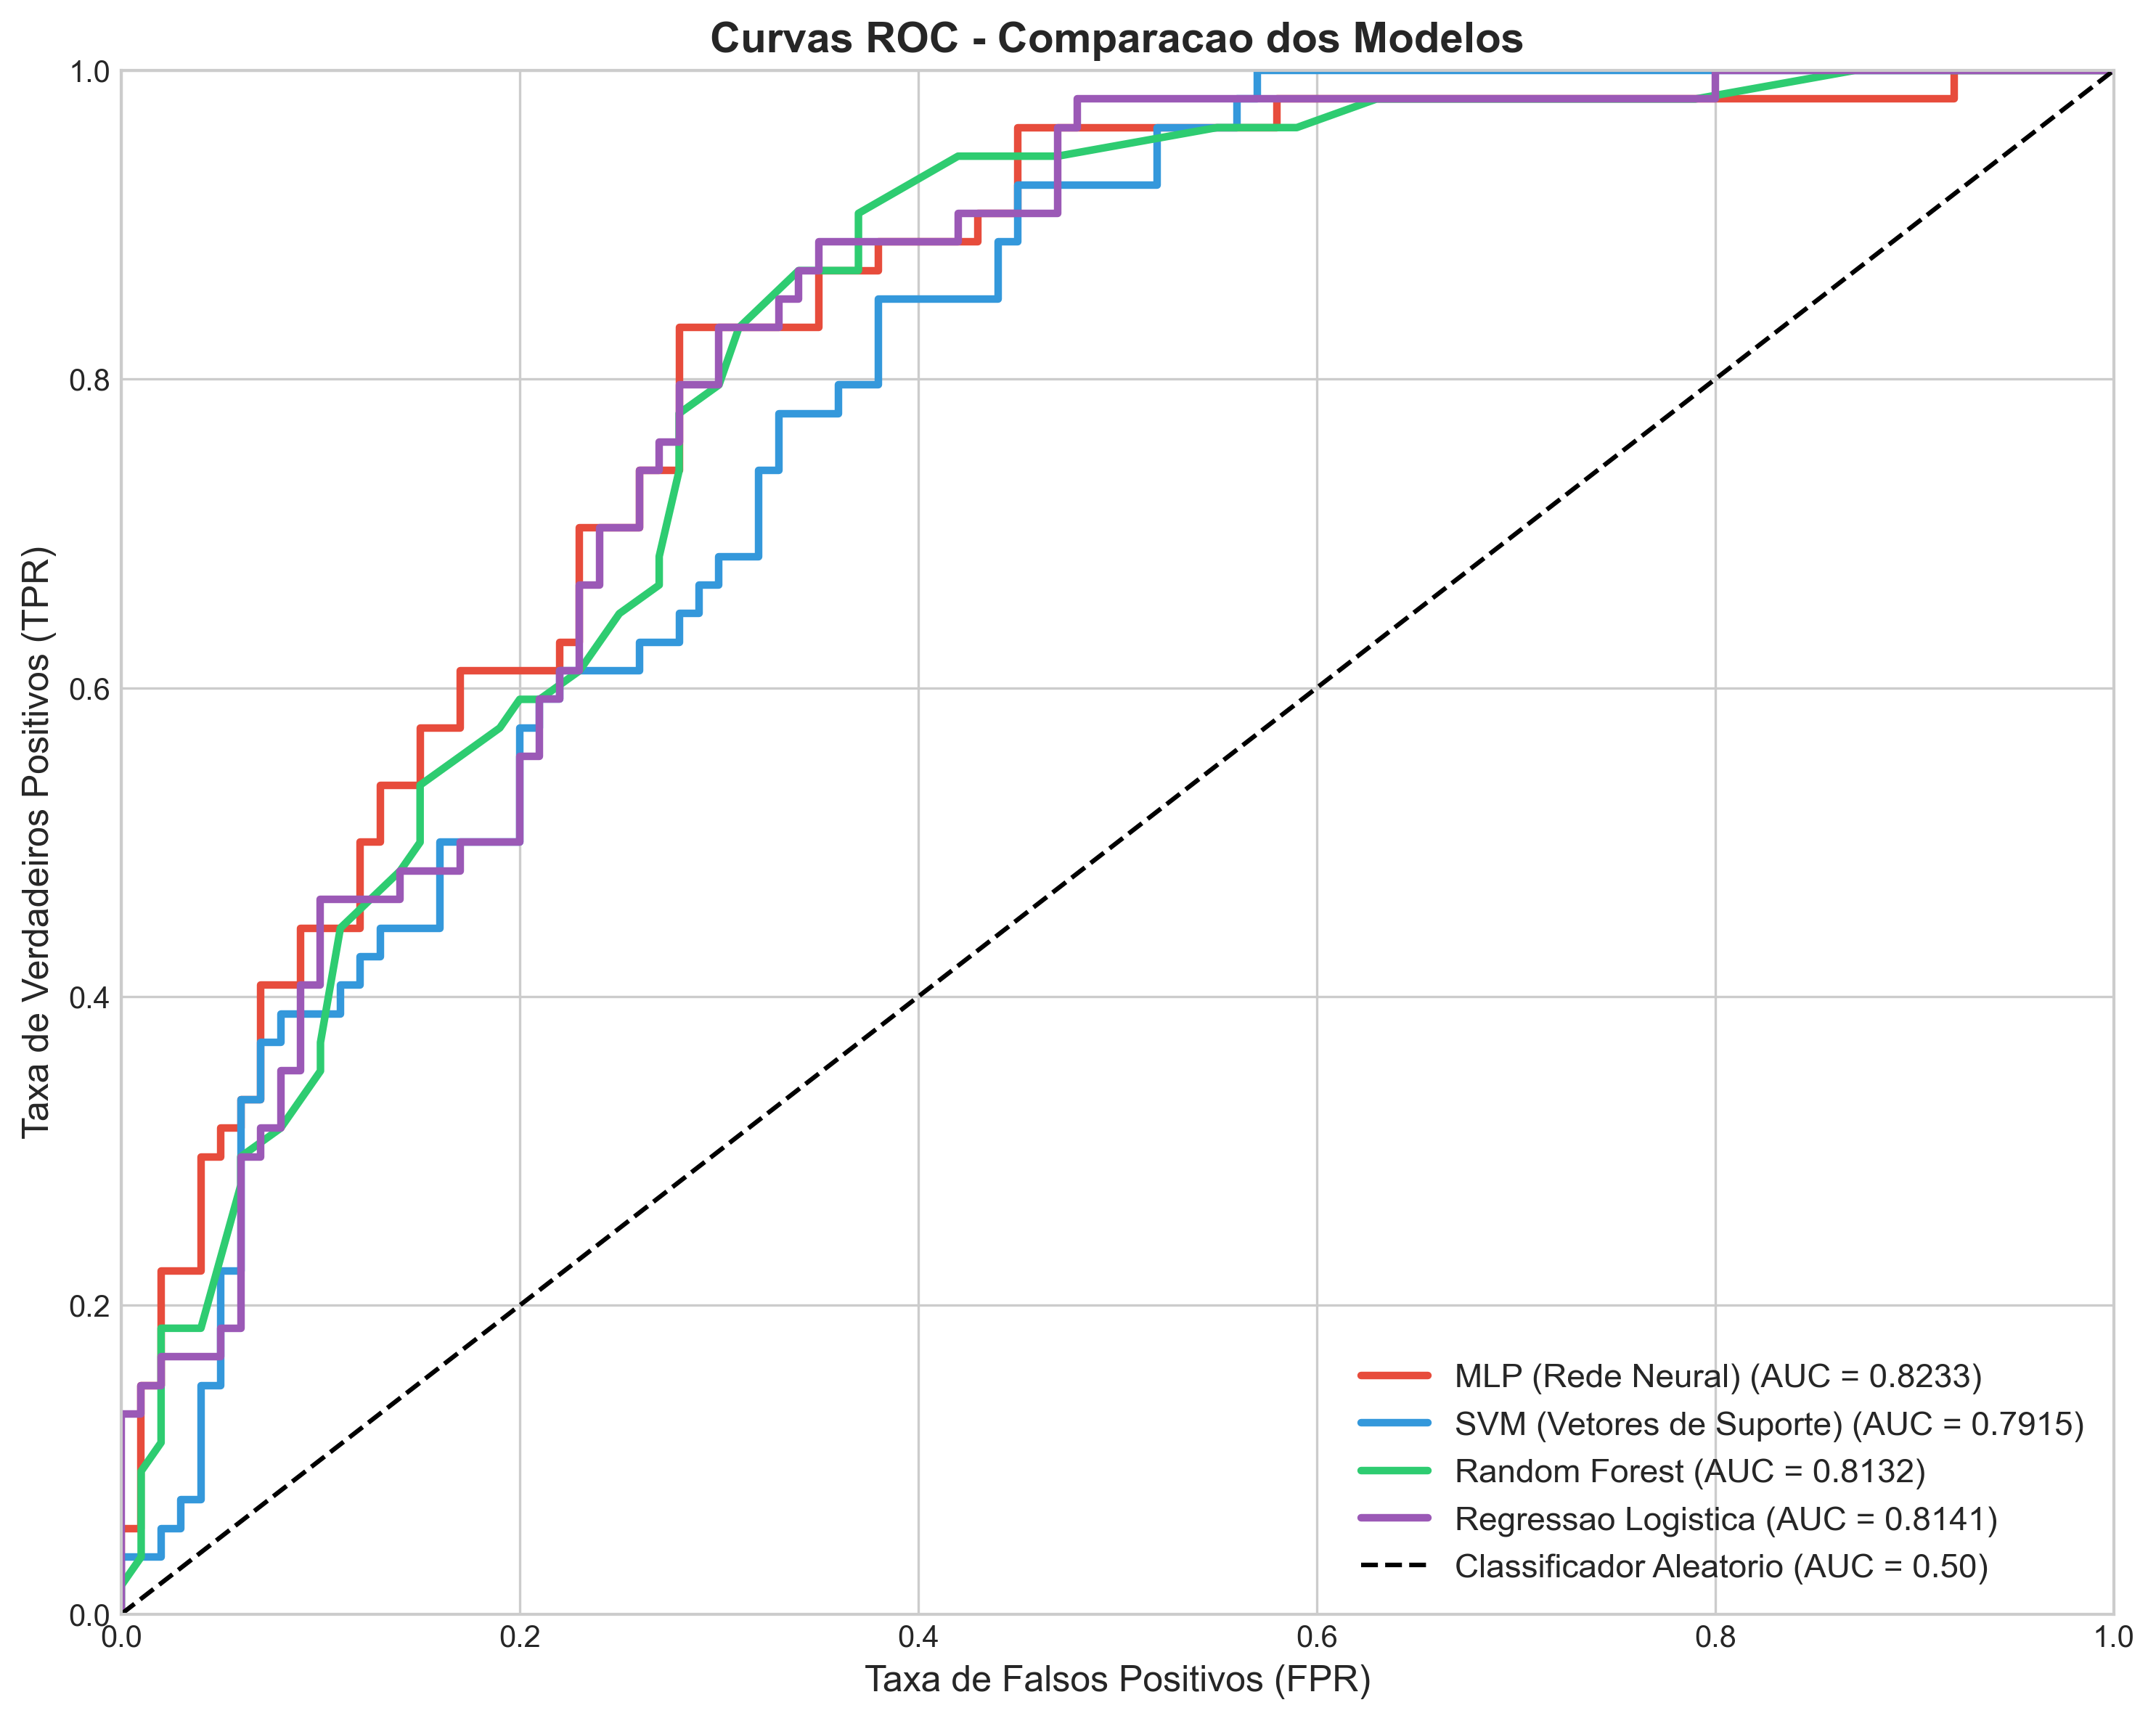
\includegraphics[width=\textwidth,height=0.45\textheight,keepaspectratio]{../figuras_diabetes/04_curvas_roc.png}
        \end{column}
        \begin{column}{0.48\textwidth}
            \centering
            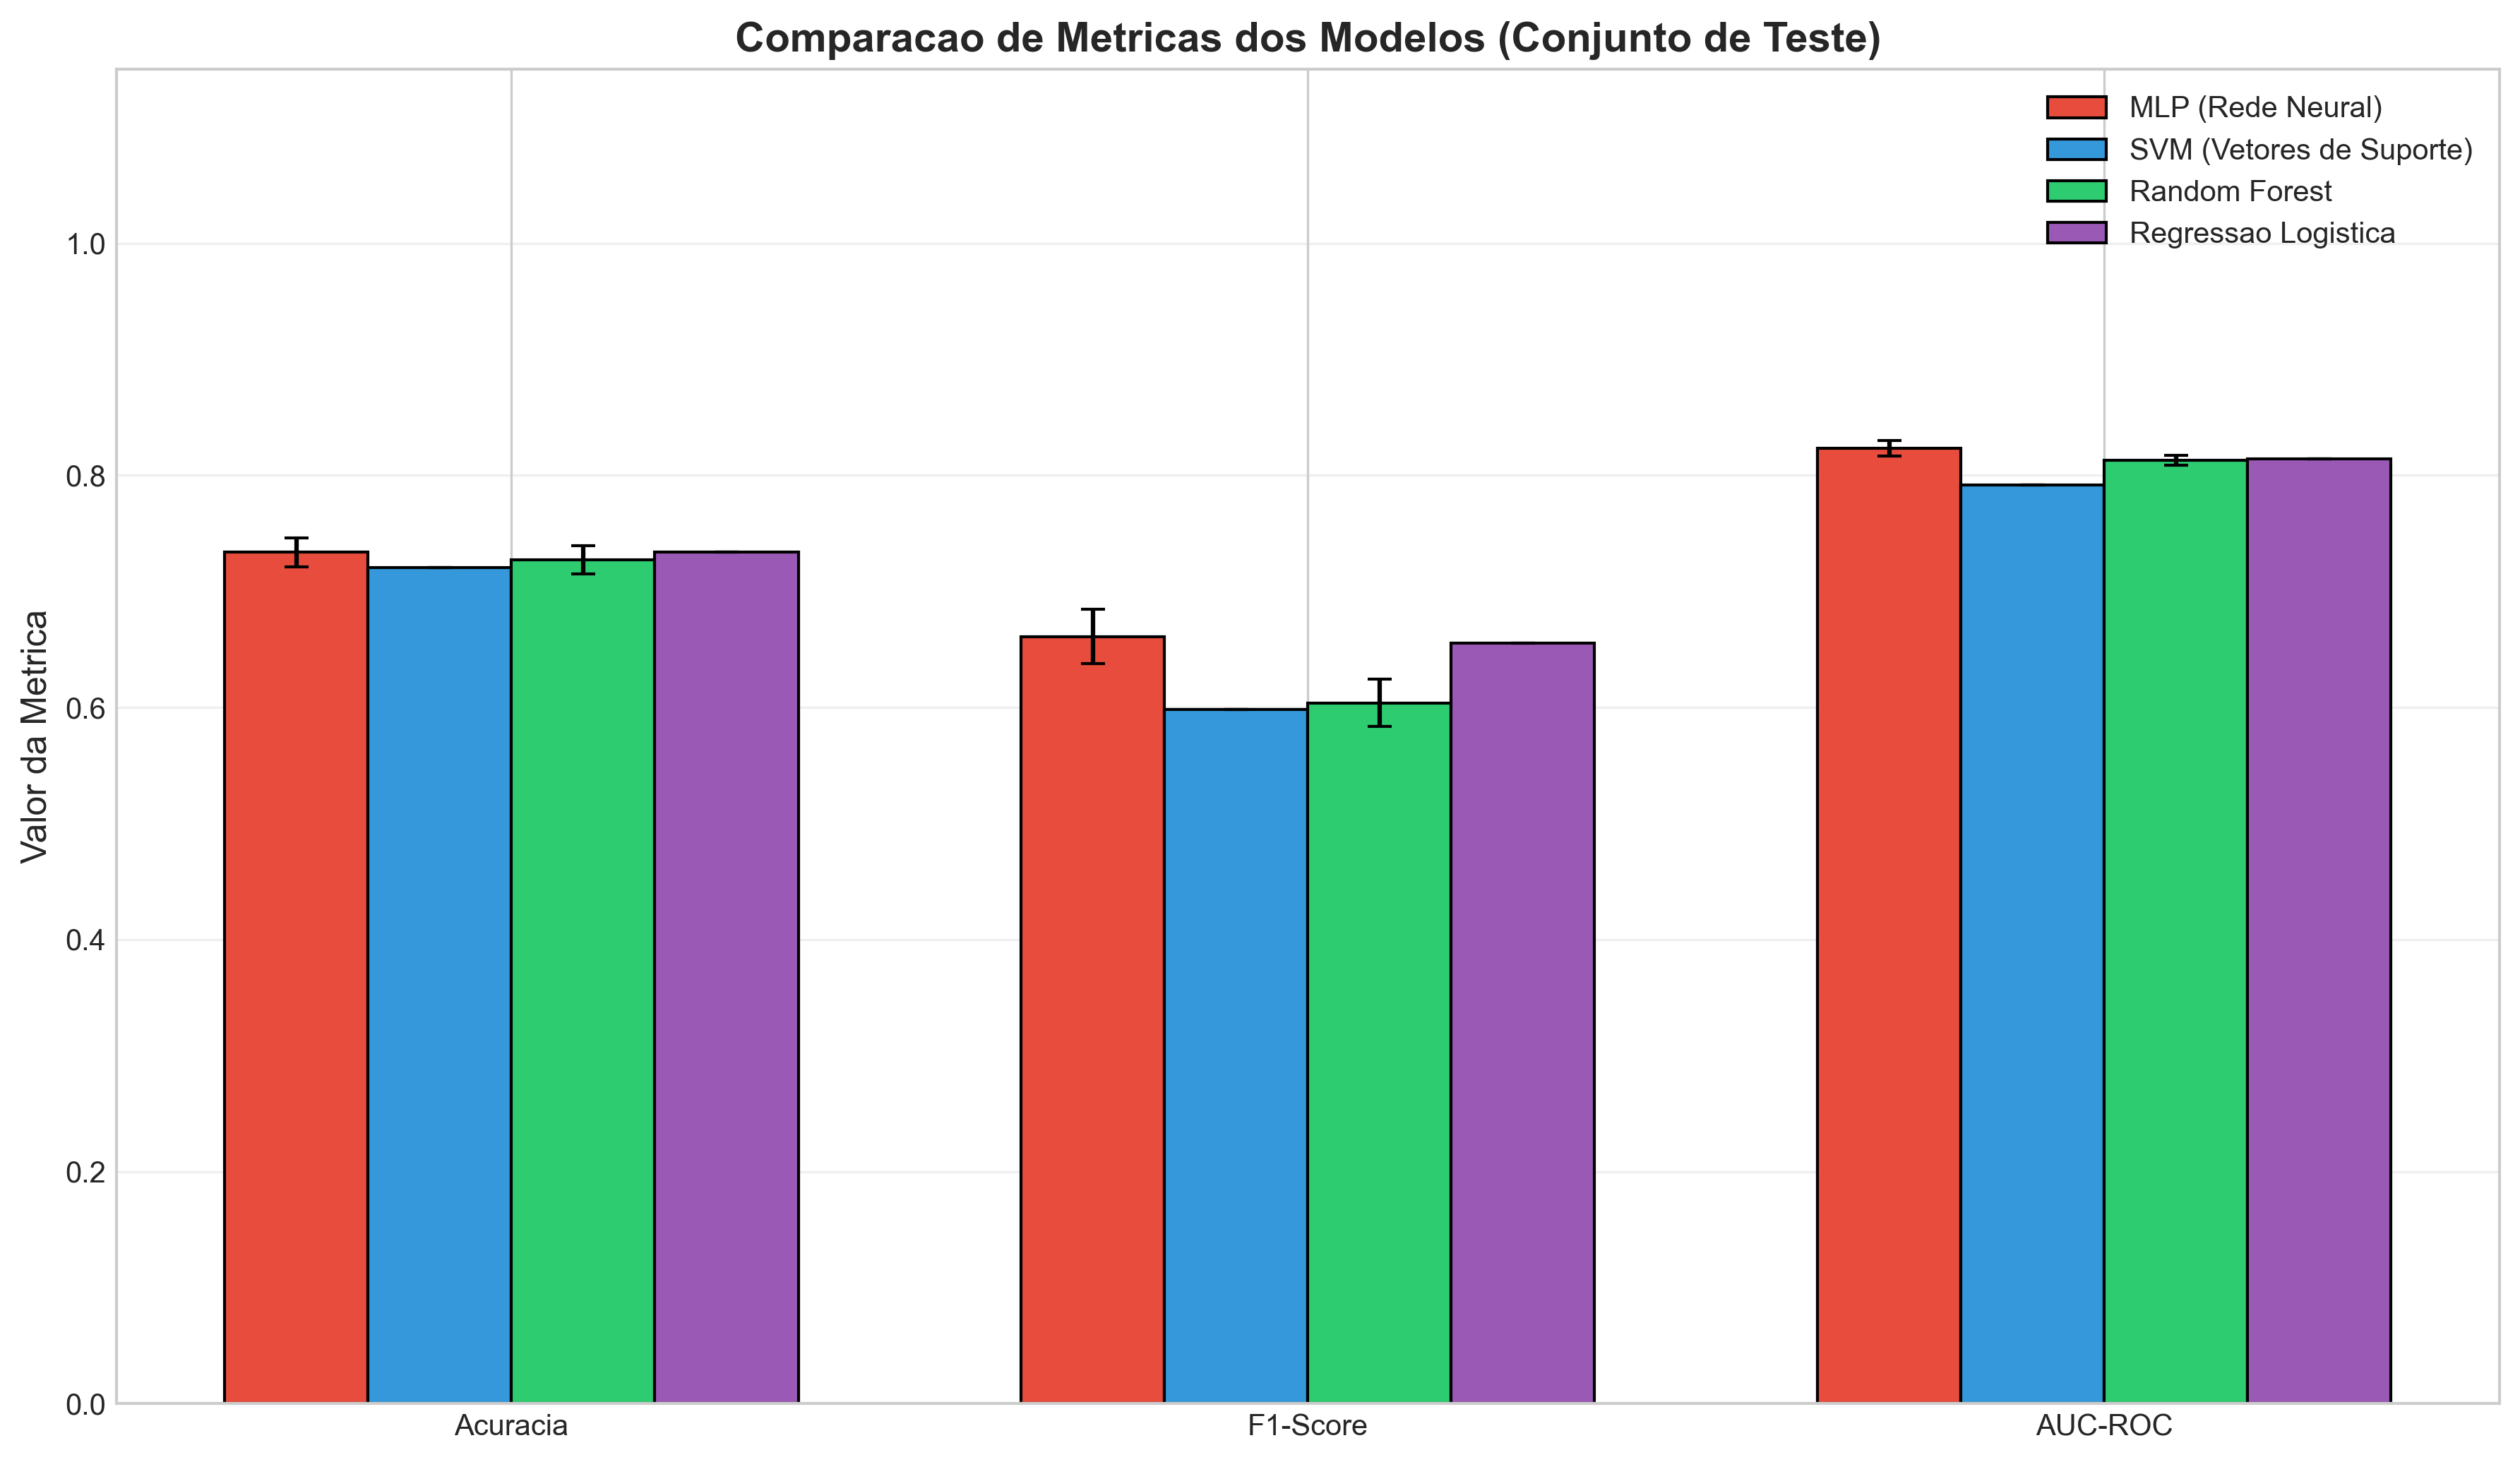
\includegraphics[width=\textwidth,height=0.45\textheight,keepaspectratio]{../figuras_diabetes/05_comparacao_metricas.png}
        \end{column}
    \end{columns}
\end{frame}

\begin{frame}{Importância das Variáveis}
    \centering
    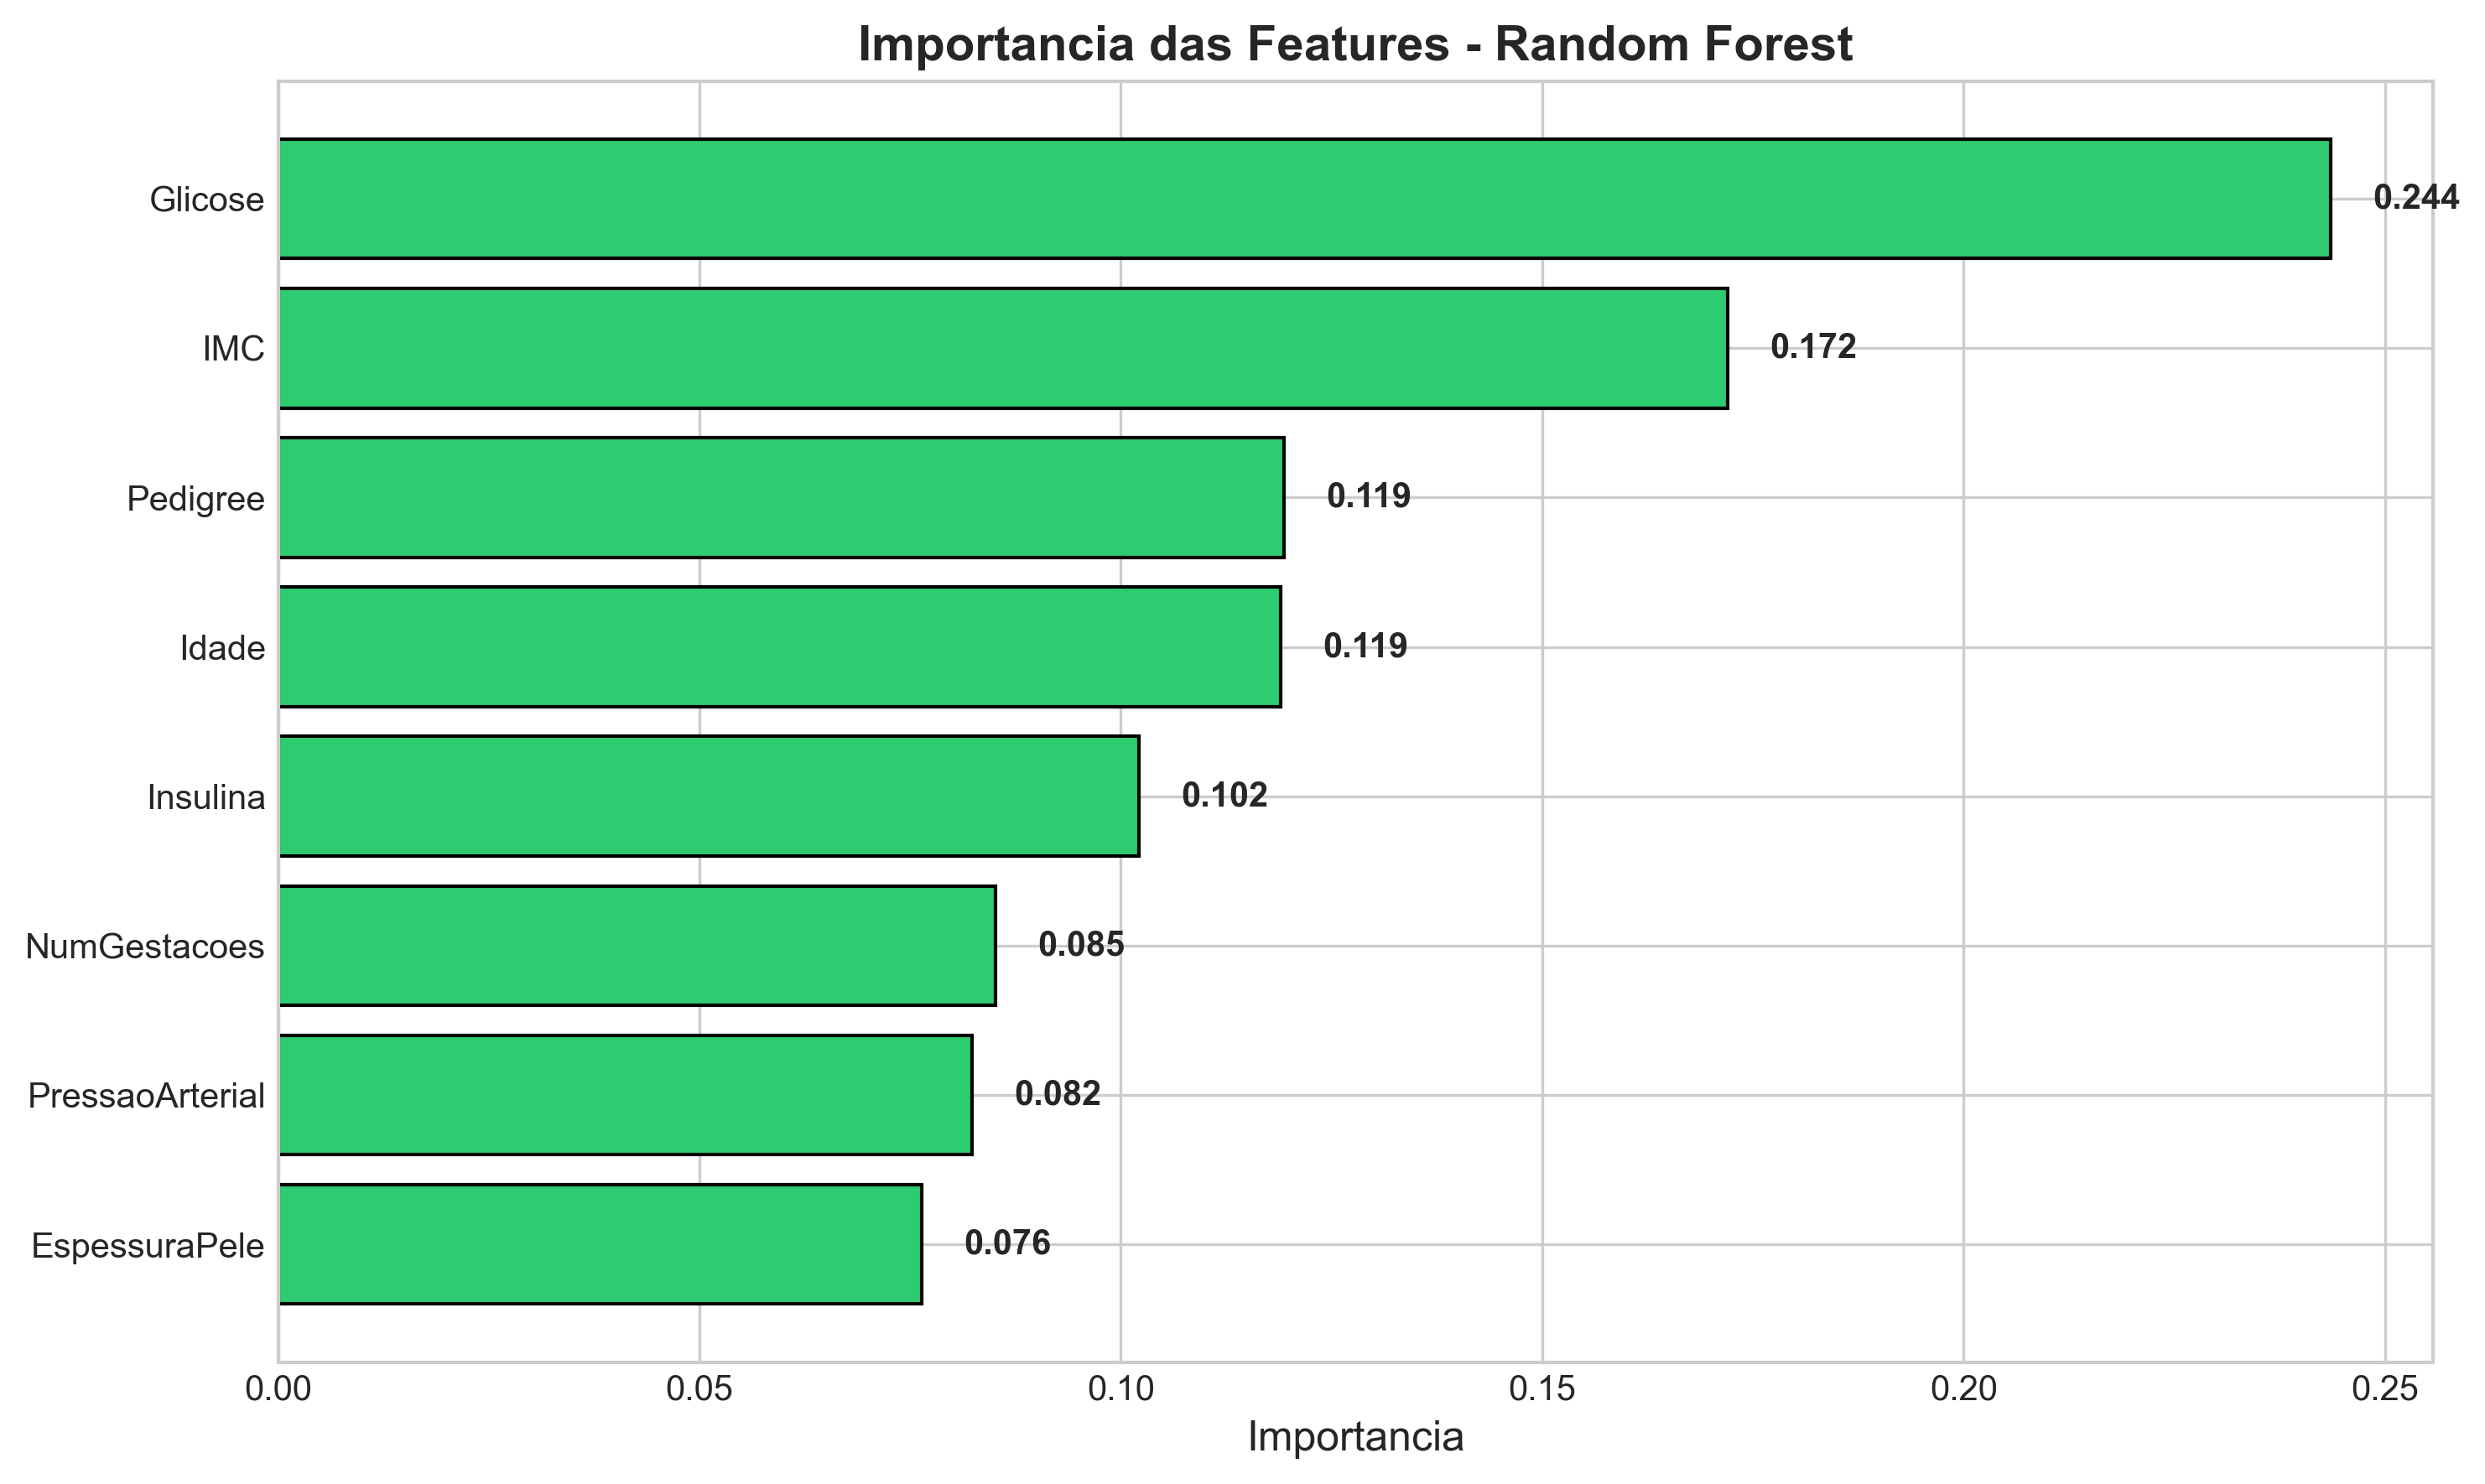
\includegraphics[width=0.95\textwidth,height=0.78\textheight,keepaspectratio]{../figuras_diabetes/07_feature_importance.png}
\end{frame}

% ================================================================
\section{Discussão e Conclusões}
% ================================================================
\begin{frame}{Discussão}
    \begin{itemize}
        \item \textbf{Regressão Logística} venceu apesar da simplicidade: escassez de dados favorece modelos com menos parâmetros e regularização adequada.
        \item \textbf{MLP} foi o segundo melhor, mas apresentou maior variabilidade entre execuções (sensibilidade à inicialização).
        \item \textbf{Random Forest} foi estável, mas limitado em magnitude; destacou Glicose e IMC como principais preditores.
        \item \textbf{SVM} obteve o menor F1; a alta regularização (C=100) pode ter causado overfitting no pequeno conjunto de treino.
        \item Todos os modelos alcançaram AUC-ROC $>$ 0,79, indicando capacidade discriminativa satisfatória.
    \end{itemize}
\end{frame}

\begin{frame}{Conclusões e Trabalhos Futuros}
    \textbf{Conclusões:}
    \begin{itemize}
        \item Pipeline completo e reprodutível de ML para predição de DMT2.
        \item Modelo mais simples (Regressão Logística) superou arquiteturas complexas neste dataset de pequeno porte.
        \item AUC-ROC superior a 0,79 para todos os modelos valida a relevância das variáveis clínicas.
    \end{itemize}
    \vspace{0.3cm}
    \textbf{Trabalhos futuros:}
    \begin{itemize}
        \item Avaliação com datasets maiores e dados hospitalares brasileiros.
        \item Exploração de modelos ensemble híbridos.
        \item Uso de técnicas de explicabilidade (SHAP, LIME) para adoção clínica.
    \end{itemize}
\end{frame}

\begin{frame}{Referências}
    \footnotesize
    \begin{thebibliography}{99}
        \bibitem{idf2021} International Diabetes Federation, ``IDF Diabetes Atlas,'' 10th ed., Brussels, 2021.
        \bibitem{kavakiotis2017} I. Kavakiotis et al., ``Machine learning and data mining methods in diabetes research,'' \emph{Comput. Struct. Biotechnol. J.}, vol. 15, pp. 104--116, 2017.
        \bibitem{haykin2009} S. Haykin, \emph{Neural Networks and Learning Machines}, 3rd ed. Pearson, 2009.
        \bibitem{smith1988} J. W. Smith et al., ``Using the ADAP learning algorithm to forecast the onset of diabetes mellitus,'' in \emph{Proc. Annu. Symp. Comput. Appl. Med. Care}, 1988, pp. 261--265.
        \bibitem{sisodia2018} D. Sisodia e D. S. Sisodia, ``Prediction of diabetes using classification algorithms,'' \emph{Procedia Comput. Sci.}, vol. 132, pp. 1578--1585, 2018.
        \bibitem{maniruzzaman2017} M. Maniruzzaman et al., ``Classification and prediction of diabetes disease using machine learning paradigm,'' \emph{Health Inf. Sci. Syst.}, vol. 5, no. 1, pp. 1--14, 2017.
    \end{thebibliography}
    \vspace{0.3cm}
    \begin{block}{Agradecimento}
        Agradecemos ao Prof. Dr. Alisson Marques da Silva pela orientação na disciplina de Inteligência Computacional.
    \end{block}
\end{frame}

\begin{frame}
    \centering
    \Huge Obrigado!
    \\[0.5cm]
    \normalsize
    Dúvidas?
    \\[0.5cm]
    \footnotesize
    \texttt{rafael.ferreira@aluno.cefetmg.br}
\end{frame}

\end{document}
